\documentclass[11pt]{ainotes}
\usepackage{xspace}

\title{Languages and Algorithms for\\Artificial Intelligence\\(Module 3)}
\date{2023 -- 2024}
\def\lastupdate{{PLACEHOLDER-LAST-UPDATE}}
\newcommand{\enc}[1]{{\llcorner{#1}\lrcorner}}
\newcommand{\tapestart}[0]{\triangleright}
\newcommand{\tapeblank}[0]{\square}
\def\P{\textbf{P}\xspace}
\def\DTIME{\textbf{DTIME}\xspace}
\def\FP{\textbf{FP}\xspace}
\def\FDTIME{\textbf{FDTIME}\xspace}
\def\EXP{\textbf{EXP}\xspace}
\def\FEXP{\textbf{FEXP}\xspace}
\def\NP{\textbf{NP}\xspace}
\def\NDTIME{\textbf{NDTIME}\xspace}

\begin{document}

    \makenotesfront
    \lohead{\color{gray} Not required for the exam}
\lehead{\color{gray} Not required for the exam}
\chapter{Introduction}


\section{AI systems classification}

\subsection{Intelligence classification}
Intelligence is defined as the ability to perceive or infer information and to retain the knowledge for future use.

\begin{description}
    \item[Weak AI] \marginnote{Weak AI}
        aims to build a system that acts as an intelligent system. 
    
        \item[Strong AI] \marginnote{Strong AI}
        aims to build a system that is actually intelligent. 
\end{description}


\subsection{Capability classification}
\begin{description}
    \item[General AI] \marginnote{General AI}
        systems able to solve any generalized task. 
    
        \item[Narrow AI] \marginnote{Narrow AI}
        systems able to solve a particular task. 
\end{description}


\subsection{AI approaches}
\begin{description}
    \item[Symbolic AI (top-down)] \marginnote{Symbolic AI}
        Symbolic representation of knowledge, understandable by humans.

    \item[Connectionist approach (bottom-up)] \marginnote{Connectionist approach}
        Neural networks. Knowledge is encoded and not understandable by humans.
\end{description}



\section{Symbolic AI}
\begin{description}
    \item[Deductive reasoning] \marginnote{Deductive reasoning}
        Conclude something given some premises (general to specific). 
        It is unable to produce new knowledge.
        \begin{example}
            "All men are mortal" and "Socrates is a man" $\rightarrow$ "Socrates is mortal"
        \end{example}
    
    \item[Inductive reasoning] \marginnote{Inductive reasoning}
        A conclusion is derived from an observation (specific to general).
        Produces new knowledge, but correctness is not guaranteed.
        \begin{example}
            "Several birds fly" $\rightarrow$ "All birds fly"
        \end{example}

    \item[Abduction reasoning] \marginnote{Abduction reasoning}
        An explanation of the conclusion is found from known premises.
        Differently from inductive reasoning, it does not search for a general rule.
        Produces new knowledge, but correctness is not guaranteed.
        \begin{example}
            "Socrates is dead" (conclusion) and "All men are mortal" (knowledge) $\rightarrow$ "Socrates is a man"
        \end{example}
    
    \item[Reasoning by analogy] \marginnote{Reasoning by analogy}
        Principle of similarity (e.g. k-nearest-neighbor algorithm).
        \begin{example}
            "Socrates loves philosophy" and Socrates resembles John $\rightarrow$ "John loves philosophy"
        \end{example}

    \item[Constraint reasoning and optimization] \marginnote{Constraint reasoning}
        Constraints, probability, statistics.
\end{description}


\section{Machine learning}

\subsection{Training approach}
\begin{description}
    \item[Supervised learning] \marginnote{Supervised learning}
        Trained on labeled data (ground truth is known).\\
        Suitable for classification and regression tasks.

    \item[Unsupervised learning] \marginnote{Unsupervised learning}
        Trained on unlabeled data (the system makes its own discoveries).\\
        Suitable for clustering and data mining.

    \item[Semi-supervised learning] \marginnote{Semi-supervised learning}
        The system is first trained to synthesize data in an unsupervised manner,
        followed by a supervised phase.

    \item[Reinforcement learning] \marginnote{Reinforcement learning}
        An agent learns by simulating actions in an environment with rewards and punishments depending on its choices.
\end{description}


\subsection{Tasks}
\begin{description}
    \item[Classification] \marginnote{Classification}
        Supervised task that, given the input variables $X$ and the output (discrete) categories $Y$,
        aims to approximate a mapping function $f: X \rightarrow Y$.

    \item[Regression] \marginnote{Regression}
        Supervised task that, given the input variables $X$ and the output (continuous) variables $Y$,
        aims to approximate a mapping function $f: X \rightarrow Y$.

    \item[Clustering] \marginnote{Clustering}
        Unsupervised task that aims to organize objects into groups.
\end{description}


\subsection{Neural networks}
\marginnote{Perceptron}
A neuron (\textbf{perceptron}) computes a weighted sum of its inputs and 
passes the result to an activation function to produce the output.
\begin{figure}[h]
    \centering
    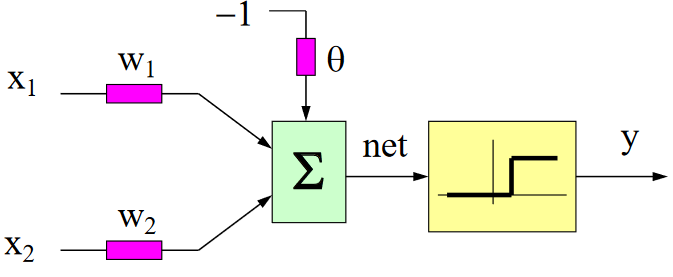
\includegraphics[width=0.40\textwidth]{img/neuron.png}
    \caption{Representation of an artificial neuron}
\end{figure}

\marginnote{Feed-forward neural network}
A \textbf{feed-forward neural network} is composed of multiple layers of neurons, each connected to the next one.
The first layer is the input layer, while the last is the output layer.
Intermediate layers are hidden layers.

The expressivity of a neural network increases when more neurons are used:
\begin{descriptionlist}
    \item[Single perceptron] 
        Able to compute a linear separation.
        \begin{figure}[h]
            \centering
            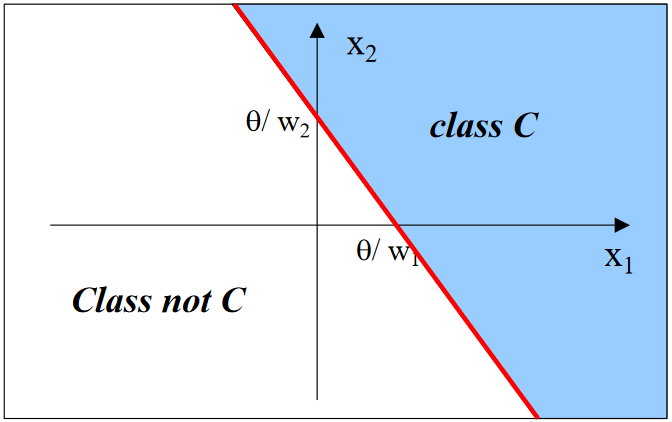
\includegraphics[width=0.25\textwidth]{img/1perceptron.png}
            \caption{Separation performed by one perceptron}
        \end{figure}
    \item[Three-layer network] 
        Able to separate a convex region ($n_\text{edges} \leq n_\text{hidden neurons}$)
        \begin{figure}[h]
            \centering
            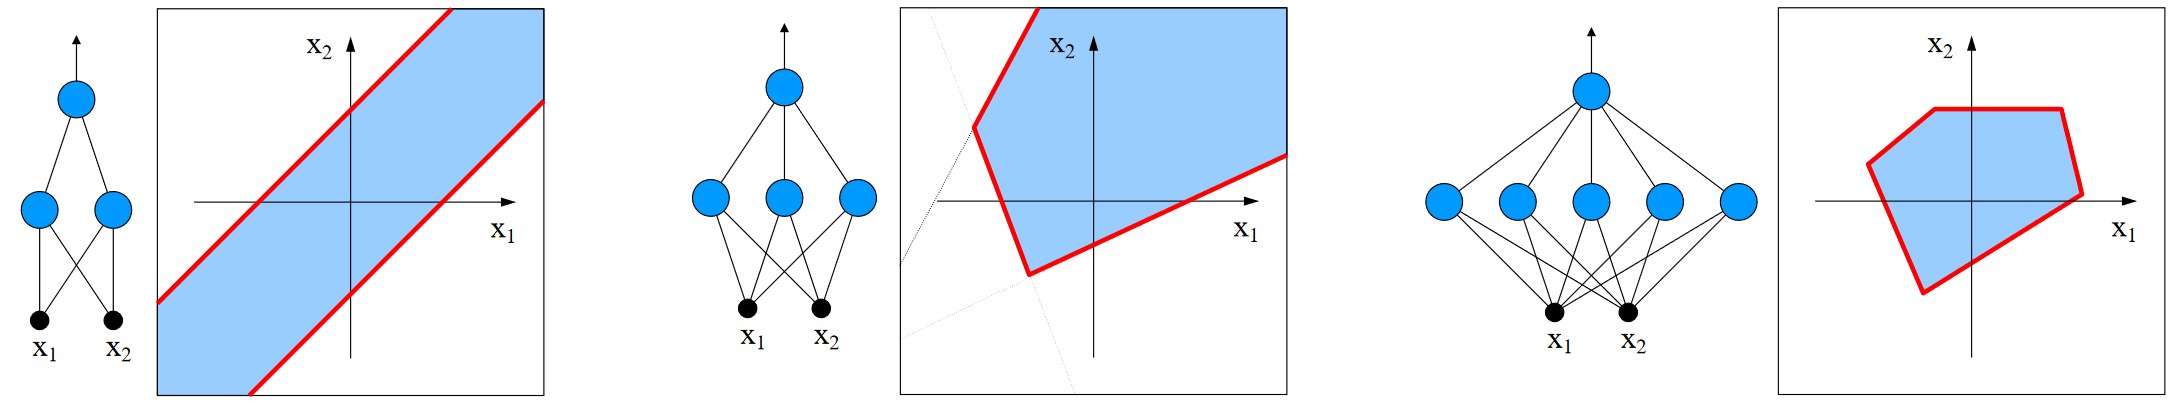
\includegraphics[width=0.90\textwidth]{img/3layer.png}
            \caption{Separation performed by a three-layer network}
        \end{figure}
    \item[Four-layer network] 
        Able to separate regions of arbitrary shape.
        \begin{figure}[h]
            \centering
            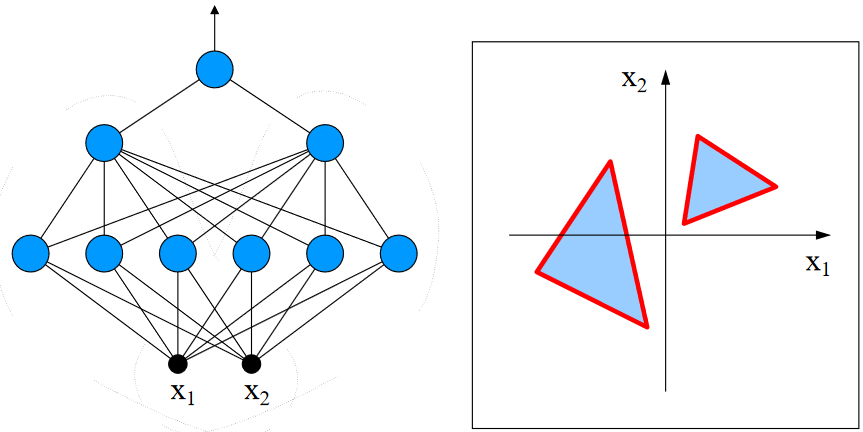
\includegraphics[width=0.40\textwidth]{img/4layer.png}
            \caption{Separation performed by a four-layer network}
        \end{figure}
\end{descriptionlist}

\begin{theorem}[Universal approximation theorem] \marginnote{Universal approximation theorem}
    A feed-forward network with one hidden layer and a finite number of neurons is
    able to approximate any continuous function with desired accuracy.
\end{theorem}

\begin{description}
    \item[Deep learning] \marginnote{Deep learning}
        Neural network with a large number of layers and neurons.
        The learning process is hierarchical: the network exploits simple features in the first layers and
        synthesizes more complex concepts while advancing through the layers.
\end{description}



\section{Automated planning}
Given an initial state, a set of actions and a goal, 
\textbf{automated planning} aims to find a partially or totally ordered sequence of actions to achieve a goal. \marginnote{Automated planning}

An \textbf{automated planner} is an agent that operates in a given domain described by:
\begin{itemize}
    \item Representation of the initial state
    \item Representation of a goal
    \item Formal description of the possible actions (preconditions and effects)
\end{itemize}



\section{Swarm intelligence}
\marginnote{Swarm intelligence}
Decentralized and self-organized systems that result in emergent behaviors. 



\section{Decision support systems}

\begin{description}
    \item[Knowledge based system] \marginnote{Knowledge based system}
        Use knowledge (and data) to support human decisions.
        Bottlenecked by knowledge acquisition.
\end{description}

Different levels of decision support exist:
\begin{descriptionlist}
    \item[Descriptive analytics] \marginnote{Descriptive analytics}
        Data are used to describe the system (e.g. dashboards, reports, \dots).
        Human intervention is required.
            
    \item[Diagnostic analytics] \marginnote{Diagnostic analytics}
        Data are used to understand causes (e.g. fault diagnosis)
        Decisions are made by humans.

    \item[Predictive analytics] \marginnote{Predictive analytics}
        Data are used to predict future evolutions of the system.
        Uses machine learning models or simulators (digital twins)

    \item[Prescriptive analytics] \marginnote{Prescriptive analytics}
        Make decisions by finding the preferred scenario.
        Uses optimization systems, combinatorial solvers or logical solvers.
\end{descriptionlist}


\newpage
\lohead{}
\lehead{}

    \chapter{Turing Machine}



\section{$k$-tape Turing Machine}

\begin{description}
    \item[Tape] \marginnote{Tape}
        Infinite one-directional line of cells.
        Each cell can hold a symbol from a finite alphabet $\Gamma$.

        \begin{description}
            \item[Tape head]
                A tape head reads or writes one symbol at a time and 
                can move left or right on the tape.

            \item[Input tape]
                Read-only tape where the input will be loaded.

            \item[Work tape]
                Read-write auxiliary tape used during computation.

            \item[Output tape]
                Read-write tape that will contain the output of the computation.

                \begin{remark}
                    Sometimes the output tape is not necessary and the final state of the computation can be used to determine a boolean outcome.
                \end{remark}
        \end{description}

    \item[Instructions] \marginnote{Instructions}
        Given a finite set of states $Q$, at each step, a machine can:
        \begin{description}
            \item[Read] from the $k$ tape heads.
            \item[Replace] the symbols under the writable tape heads, or leave them unchanged.
            \item[Change] state.
            \item[Move] each of the $k$ tape heads to the left or right, or leave unchanged.
        \end{description}


    \item[$k$-tape Turing Machine (TM)] \marginnote{$k$-tape Turing Machine (TM)}
        A Turing Machine working on $k$ tapes (one of which is the input tape) is a triple $(\Gamma, Q, \delta)$:
        \begin{itemize}
            \item $\Gamma$ is a finite set of tape symbols.
                We assume that it contains a blank symbol ($\tapeblank$), a start symbol ($\tapestart$),
                and the digits $0$, $1$.
            
            \item $Q$ is a finite set of states.
                The initial state is $q_\text{init}$ and the final state is $q_\text{halt}$.

            \item $\delta$ is the transition function that describes the instructions allowed at each step. 
                It is defined as:
                \[ \delta: Q \times \Gamma^k \rightarrow Q \times \Gamma^{k-1} \times \{ \texttt{L}, \texttt{S}, \texttt{R} \}^k \]

                By convention, when the state is $q_\text{halt}$, the machine is stuck (i.e. it cannot change state or operate on the tapes):
                \[ \delta(q_\text{halt}, \{ \sigma_1, \dots, \sigma_k \}) = \big( q_\text{halt}, \{ \sigma_1, \dots, \sigma_k \}, (\texttt{S}, \dots, \texttt{S}) \big) \]
        \end{itemize}
\end{description}

\begin{theorem}[Turing Machine equivalence]
    The following computational models have, with at most a polynomial overhead, the same expressive power:
    1-tape TMs, $k$-tape TMs, non-deterministic TMs, 
    random access machines, $\lambda$-calculus, unlimited register machines, programming languages (Böhm-Jacopini theorem), \dots
\end{theorem}



\section{Computation}

\begin{description}
    \item[Configuration] \marginnote{Configuration}
        Given a TM $\mathcal{M} = (\Gamma, Q, \delta)$, a configuration $C$ is described by:
        \begin{itemize}
            \item The current state $q$.
            \item The content of the tapes.
            \item The position of the tape heads.
        \end{itemize}

        \begin{description}
            \item[Initial configuration] 
                Given the input $x \in \{ 0, 1 \}^*$, the initial configuration $\mathcal{I}_x$ is described as follows:
                \begin{itemize}
                    \item The current state is $q_\text{init}$.
                    \item The first (input) tape contains $\tapestart x \tapeblank \dots$.
                        The other tapes contain $\tapestart \tapeblank \dots$.
                    \item The tape heads are positioned on the first symbol of each tape.
                \end{itemize}

            \item[Final configuration] 
                Given an output $y \in \{0, 1\}^*$, the final configuration is described as follows:
                \begin{itemize}
                    \item The current state is $q_\text{halt}$.
                    \item The output tape contains $\tapestart y \tapeblank \dots$.
                \end{itemize} 
        \end{description}

    \item[Computation (string)] \marginnote{Computation (string)}
        Given a TM $\mathcal{M} = (\Gamma, Q, \delta)$, 
        $\mathcal{M}$ returns $y \in \{ 0, 1 \}^*$ on input $x \in \{ 0, 1 \}^*$ (i.e. $\mathcal{M}(x) = y$) in $t$ steps if:
        \[ \mathcal{I}_x \xrightarrow{\delta} C_1 \xrightarrow{\delta} \dots \xrightarrow{\delta} C_t \]
        where $C_t$ is a final configuration for $y$.

    \item[Computation (function)] \marginnote{Computation (function)}
        Given a TM $\mathcal{M} = (\Gamma, Q, \delta)$ and a function $f: \{0, 1\}^* \rightarrow \{0, 1\}^*$, 
        $\mathcal{M}$ computes $f$ iff:
        \[ \forall x \in \{0, 1\}^*: \mathcal{M}(x) = f(x) \]
        If this holds, $f$ is a computable function.

    \item[Computation in time $\mathbf{T}$] \marginnote{Computation in time $T$}
        Given a TM $\mathcal{M}$ and 
        the functions $f: \{0, 1\}^* \rightarrow \{0, 1\}^*$ and
        $T: \mathbb{N} \rightarrow \mathbb{N}$,
        $\mathcal{M}$ computes $f$ in time $T$ iff:
        \[ \forall x \in \{0, 1\}^*: \text{$\mathcal{M}(x)$ returns $f(x)$ in at most $T(\vert x \vert)$ steps} \]

    \item[Decidability in time $\mathbf{T}$] \marginnote{Decidability in time $T$}
        Given a function $f: \{0, 1\}^* \rightarrow \{0, 1\}$,
        the language $\mathcal{L}_f$ is decidable in time $T$ iff $f$ is computable in time $T$.
\end{description}



\section{Universal Turing Machine}

\begin{description}
    \item[Turing Machine encoding]
        Given a TM $\mathcal{M} = (\Gamma, Q, \delta)$, 
        the entire machine can be described by $\delta$ through tuples of form:
        \[ Q \times \Gamma^k \times Q \times \Gamma^{k-1} \times \{ \texttt{L}, \texttt{S}, \texttt{R} \}^k \]
        It is therefore possible to encode $\delta$ into a binary string and 
        consequently create an encoding $\enc{\mathcal{M}}$ of $\mathcal{M}$.

        The encoding should satisfy the following conditions:
        \begin{enumerate}
            \item For every $x \in \{0, 1\}^*$, there exists a TM $\mathcal{M}$ such that $x = \enc{\mathcal{M}}$.
            \item Every TM is represented by an infinite number of strings. One of them is the canonical representation.
        \end{enumerate}

    \begin{theorem}[Universal Turing Machine (UTM)] \marginnote{Universal Turing Machine (UTM)}
        There exists a TM $\mathcal{U}$ such that, for every binary strings $x$ and $\alpha$,
        it emulates the TM defined by $\alpha$ on input $x$:
        \[ \mathcal{U}(x, \alpha) = \mathcal{M}_\alpha(x) \]
        where $\mathcal{M}_\alpha$ is the TM defined by $\alpha$.

        Moreover, $\mathcal{U}$ simulates $\mathcal{M}_\alpha$ with at most $CT\log(T)$ time overhead,
        where $C$ only depends on $\mathcal{M}_\alpha$.
    \end{theorem}
\end{description}



\section{Computability}


\subsection{Undecidable functions}

\begin{theorem}[Existance of uncomputable functions] \label{th:uncomputable_fn} \marginnote{Uncomputable functions}
    There exists a function $uc: \{0, 1\}^* \rightarrow \{0, 1\}^*$ that is not computable by any TM.

    \begin{proof}
        Consider the following function:
        \[ uc(\alpha) = \begin{cases}
            0 & \text{if $\mathcal{M}_\alpha(\alpha) = 1$} \\
            1 & \text{if $\mathcal{M}_\alpha(\alpha) \neq 1$}
        \end{cases} \]
        If $uc$ was computable, there would be a TM $\mathcal{M}$ that computes it (i.e. $\forall \alpha \in \{0, 1\}^*: \mathcal{M}(\alpha) = uc(\alpha)$).
        This will result in a contradiction:
        \[ uc(\enc{\mathcal{M}}) = 0 \iff \mathcal{M}(\enc{\mathcal{M}}) = 1 \iff uc(\enc{\mathcal{M}}) = 1 \]

        Therefore, $uc$ cannot be computed.
    \end{proof}
\end{theorem}


\begin{description}
    \item[Halting problem] \marginnote{Halting problem}
        Given an encoded TM $\alpha$ and a string $x$,
        the halting problem aims to determine if $\mathcal{M}_\alpha$ terminates on input $x$.
        In other words:
        \[
            \texttt{halt}(\enc{(\alpha, x)}) = \begin{cases}
                1 & \text{if $\mathcal{M}_\alpha$ stops on input $x$} \\
                0 & \text{otherwise}
            \end{cases}  
        \]
        \begin{theorem}
            The halting problem is undecidable.
        
            \begin{proof}
                Note: this proof is slightly different from the traditional proof of the halting problem.
                
                Assume that \texttt{halt} is decidable. Therefore, there exists a TM $\mathcal{M}_\texttt{halt}$ that decides it.

                We can define a new TM $\mathcal{M}_{uc}$ that uses $\mathcal{M}_\texttt{halt}$ such that:
                \[ \mathcal{M}_{uc}(\alpha) = \begin{cases}
                    1 & \text{if $\mathcal{M}_\texttt{halt}(\alpha, \alpha) = 0$ (i.e. $\mathcal{M}_\alpha(\alpha)$ diverges)} \\
                    \begin{cases}
                        0 & \text{if $\mathcal{M}_\alpha(\alpha) = 1$} \\
                        1 & \text{if $\mathcal{M}_\alpha(\alpha) \neq 1$}
                    \end{cases} & \text{if $\mathcal{M}_\texttt{halt}(\alpha, \alpha) = 1$ (i.e. $\mathcal{M}_\alpha(\alpha)$ converges)}
                \end{cases} \]

                This results in a contradiction:
                \begin{itemize}
                    \item $\mathcal{M}_{uc}(\enc{\mathcal{M}_{uc}}) = 1 \Leftarrow 
                        \mathcal{M}_\texttt{halt}(\enc{\mathcal{M}_{uc}}, \enc{\mathcal{M}_{uc}}) = 0 \iff
                        \mathcal{M}_{uc}(\enc{\mathcal{M}_{uc}}) \text{ diverges}$
                    \item $\mathcal{M}_\texttt{halt}(\enc{\mathcal{M}_{uc}}, \enc{\mathcal{M}_{uc}}) = 1$ $\Rightarrow$
                        $\mathcal{M}_{uc}$ is not computable by \Cref{th:uncomputable_fn}.
                \end{itemize}
            \end{proof}
        \end{theorem}

    \item[Diophantine equation] \marginnote{Diophantine equation}
        Polynomial equality with integer coefficients and a finite number of unknowns.

        \begin{theorem}[MDPR]
            Determining if an arbitrary diophantine equation has a solution is undecidable.
        \end{theorem}
\end{description}



\subsection{Rice's theorem}

\begin{description}
    \item[Semantic language] \marginnote{Semantic language}
        Given a language $\mathcal{L} \subseteq \{ 0, 1 \}^*$, $\mathcal{L}$ is semantic if:
        \begin{itemize}
            \item Any string in $\mathcal{L}$ is an encoding of a TM.
            \item If $\enc{\mathcal{M}} \in \mathcal{L}$ and 
                the TM $\mathcal{N}$ computes the same function of $\mathcal{M}$,
                then $\enc{\mathcal{N}} \in \mathcal{L}$.
        \end{itemize}

        A semantic language can be seen as a set of TMs that have the same property.

    \item[Trivial language]
        A language $\mathcal{L}$ is trivial iff $\mathcal{L} = \varnothing$ or $\mathcal{L} = \{0, 1\}^*$
\end{description}

\begin{theorem}[Rice's theorem] \marginnote{Rice's theorem}
    If a semantic language is non-trivial, then it is undecidable
    (i.e. any decidable semantic language is trivial).

    \begin{proof}[Proof idea]
        Assuming that there exists a non-trivial decidable semantic language $\mathcal{L}$, 
        it is possible to prove that the halting problem is decidable.
        Therefore, $\mathcal{L}$ is undecidable.
    \end{proof}
\end{theorem}
    \chapter{Complexity}


\begin{description}
    \item[Complexity class] \marginnote{Complexity class}
        Set of tasks that can be computed within some fixed resource bounds.
\end{description}



\section{Polynomial time}

\begin{description}
    \item[Deterministic time (\DTIME)] \marginnote{Deterministic time (\DTIME)}
        Let $T: \mathbb{N} \rightarrow \mathbb{N}$ and $\mathcal{L}$ be a language.
        $\mathcal{L}$ is in $\DTIME(T(n))$ iff
        there exists a TM that decides $\mathcal{L}$ in time $O(T(n))$.

    \item[Polynomial time (\P)] \marginnote{Polynomial time (\P)}
        The class \P contains all the tasks computable in polynomial time:
        \[ \P = \bigcup_{c \geq 1} \DTIME(n^c) \]

        \begin{remark}
            \P is closed to various operations on programs (e.g. composition of programs)
        \end{remark}

        \begin{remark}
            In practice, the exponent is often small.
        \end{remark}

        \begin{remark}
            \P considers the worst case and is not always realistic.
            Other alternative computational models exist.
        \end{remark}
    
    \item[Church-Turing thesis] \marginnote{Church-Turing thesis}
        Any physically realizable computer can be simulated by a TM with an arbitrary time overhead.

    \item[Strong Church-Turing thesis] \marginnote{Strong Church-Turing thesis}
        Any physically realizable computer can be simulated by a TM with a polynomial time overhead.

        \begin{remark}
            If this thesis holds, the class \P is robust 
            (i.e. does not depend on the computational device)
            and is therefore the smallest class of bounds.
        \end{remark}

    \item[Deterministic time for functions (\FDTIME)] \marginnote{Deterministic time for functions (\FDTIME)}
        Let $T: \mathbb{N} \rightarrow \mathbb{N}$ and 
        $f: \{0, 1\}^* \rightarrow \{0, 1\}^*$.
        $f$ is in $\FDTIME(T(n))$ iff
        there exists a TM that computes it in time $O(T(n))$.

    \item[Polynomial time for functions (\FP)] \marginnote{Polynomial time for functions (\FP)}
        The class \FP is defined as:
        \[ \FP = \bigcup_{c \geq 1} \FDTIME(n^c) \]
        
        \begin{remark}
            It holds that $\forall \mathcal{L} \in \P \Rightarrow f_\mathcal{L} \in \FP$,
            where $f_\mathcal{L}$ is the characteristic function of $\mathcal{L}$.
            Generally, the contrary does not hold.
        \end{remark}
\end{description}



\section{Exponential time}

\begin{description}
    \item[Exponential time (\EXP/\FEXP)] \marginnote{Exponential time (\EXP/\FEXP)}
        The \EXP and \FEXP classes are defined as:
        \[
            \EXP = \bigcup_{c \geq 1} \DTIME\big( 2^{n^c} \big) \hspace{3em} 
            \FEXP = \bigcup_{c \geq 1} \FDTIME\big( 2^{n^c} \big)
        \]

        \begin{theorem}
            The following hold:
            \[ \P \subset \EXP \hspace{3em} \FP \subset \FEXP \]
        \end{theorem}
\end{description}
    \chapter{Computational learning theory}

\begin{description}
    \item[Instance space] \marginnote{Instance space}
        Set $X$ of (encoded) instances of objects that a learner wants to classify.

        Data from the instance space is drawn from a distribution $\mathcal{D}$ unknown to the learner.

    \item[Concept] \marginnote{Concept}
        Subset $c \subseteq X$ of the instance space which can be intended as properties of objects (i.e. a way to classify the instance space).

    \item[Concept class] \marginnote{Concept class}
        Collection $\mathcal{C} \subseteq \mathbb{P}(X)$ of concepts.

        It represents the concepts that are sufficiently simple for the algorithm to handle (i.e. the space of learnable concepts).

        \begin{description}
            \item[Target concept]
                Concept $c \in \mathcal{C}$ that the learner wants to learn.
        \end{description}

        \begin{remark}
            A learning algorithm is designed to learn concepts from a concept class
            neither knowing the target concept nor its data distribution.
        \end{remark}

    \item[Learning algorithm] \marginnote{Learning algorithm}
        Given a concept class $\mathcal{C}$ and a target concept $c \in \mathcal{C}$ with unknown distribution $\mathcal{D}$, 
        a learning algorithm $\mathcal{A}$ takes as input:
        \begin{itemize}
            \item $\varepsilon$, the error parameter (or accuracy if seen as $(1-\varepsilon)$),
            \item $\delta$, the confidence parameter,
            \item $EX(c, \mathcal{D})$, an oracle that $\mathcal{A}$ can call to retrieve a data point $x \sim \mathcal{D}$ 
                with a label to indicate whether it is in the target concept $c$ or not (i.e. training data),
        \end{itemize}
        and outputs a concept $h \in \mathcal{C}$. 
        \begin{center}
            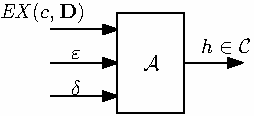
\includegraphics[width=0.3\linewidth]{./img/_learning_algorithm.pdf}
        \end{center}

        \begin{description}
            \item[Probability of error] \marginnote{Probability of error}
                Given a concept class $\mathcal{C}$, 
                a target concept $c \in \mathcal{C}$ with unknown distribution $\mathcal{D}$ and 
                a learning algorithm $\mathcal{A}$,
                the probability of error (i.e. misclassifications) for any output $h \in \mathcal{C}$ of $\mathcal{A}$ is defined as:
                \[ \text{error}_{\mathcal{D}, c} = \mathcal{P}_{x \sim \mathcal{D}}[ h(x) \neq c(x) ] \]
        \end{description}

        \begin{figure}[H]
            \centering
            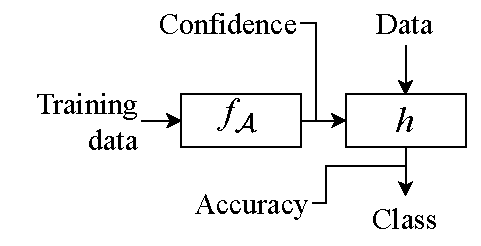
\includegraphics[width=0.35\linewidth]{./img/_learning_model.pdf}
            \caption{General idea of a learning algorithm $\mathcal{A}$ computed as a function $f_\mathcal{A}$}
        \end{figure}

    \item[PAC learnability] \marginnote{PAC learnability}
        A concept class $\mathcal{C}$ over the instance space $X$ is probably approximately correct (PAC) learnable iff there is an algorithm $\mathcal{A}$ such that:
        \begin{itemize}
            \item For each target concept $c \in \mathcal{C}$,
            \item For each distribution $\mathcal{D}$, 
            \item For each error $0 < \varepsilon < \frac{1}{2}$,
            \item For each confidence $0 < \delta < \frac{1}{2}$,
        \end{itemize}
        it holds that:
        \[ \mathcal{P}\left[ \text{error}_{\mathcal{D}, c}\Big( \mathcal{A}\big( EX(c, \mathcal{D}), \varepsilon, \delta \big) \Big) < \varepsilon \right] > 1-\delta \]
        where the probability is computed by sampling data points from $EX(c, \mathcal{D})$.

        In other words, the probability that $\mathcal{A}$ has an error rate lower than $\varepsilon$ (or an accuracy higher than $(1-\varepsilon)$) is greater than $(1-\delta)$.

        \begin{description}
            \item[Efficient PAC learnability] \marginnote{Efficient PAC learnability}
                A concept class $\mathcal{C}$ is efficiently PAC learnable iff
                it is PAC learnable and the algorithm $\mathcal{A}$ that learns it has 
                a time complexity bound to a polynomial in $\frac{1}{\varepsilon}$ and $\frac{1}{\delta}$.

                \begin{remark}
                    The complexity of $\mathcal{A}$ is measured taking into account the number of calls to $EX(c, \mathcal{D})$.
                \end{remark}
        \end{description}
\end{description}

\begin{example}[Axes-aligned rectangles in $\mathbb{R}^2_{[0, 1]}$]
    Consider the instance space $X = \mathbb{R}^2_{[0, 1]}$
    and the concept class $\mathcal{C}$ of concepts represented by all the points contained within a rectangle parallel to the axes of arbitrary size.

    \begin{figure}[H]
        \centering
        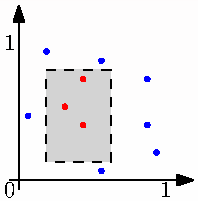
\includegraphics[width=0.2\linewidth]{./img/_learning_rectangle.pdf}
        \caption{Example of problem instance. The gray rectangle is the target concept, red dots are positive data points and blue dots are negative data points.}
    \end{figure}

    An algorithm has to guess a classifier (i.e. a rectangle) without knowing the target concept and the distribution of its training data.
    Let an algorithm $\mathcal{A}_\text{BFP}$ be defined as follows:
    \begin{itemize}
        \item Take as input some data $\{ ((x_1, y_1), p_1), \dots, ((x_n, y_n), p_n) \}$ where 
            $(x_i, y_i)$ are the coordinates of the point and $p_i$ indicates if the point is within the target rectangle.
        \item Return the smallest rectangle that includes all the positive instances.
    \end{itemize}

    Given the rectangle $R$ predicted by $\mathcal{A}_\text{BFP}$ and the target rectangle $T$,
    the probability of error in using $R$ in place of $T$ is:
    \[ \text{error}_{\mathcal{D}, T}(R) = \mathcal{P}_{x \sim \mathcal{D}} [ x \in (R \smallsetminus T) \cup (T \smallsetminus R) ] \]
    In other words, a point is misclassified if it is in $R$ but not in $T$ or vice versa.
    \begin{remark}
        By definition of $\mathcal{A}_\text{BFP}$, it always holds that $R \subseteq T$. 
        Therefore, $(R \smallsetminus T) = \varnothing$ and the error can be rewritten as:
        \[ \text{error}_{\mathcal{D}, T}(R) = \mathcal{P}_{x \sim \mathcal{D}} [ x \in (T \smallsetminus R) ] \]
    \end{remark}


    \begin{theorem}[Axes-aligned rectangles in $\mathbb{R}^2_{[0, 1]}$ PAC learnability]
        It holds that:
        \begin{itemize}
            \item For every distribution $\mathcal{D}$,
            \item For every error $0 < \varepsilon < \frac{1}{2}$, 
            \item For every confidence $0 < \delta < \frac{1}{2}$,
        \end{itemize} 
        if $m \geq \frac{4}{\varepsilon}\ln\left( \frac{4}{\delta} \right)$, then:
        \[ 
            \mathcal{P}_{D \sim \mathcal{D}^m}
                \left[ \text{error}_{\mathcal{D}, T}\Big( \mathcal{A}_\text{BFP}\big(T(D)\big) \Big) < \varepsilon \right]  > 1 - \delta
        \]
        where $D \sim \mathcal{D}^m$ is a sample of $m$ data points (i.e. training data)
        and $T(\cdot)$ labels the input data wrt to the target rectangle $T$.

        \begin{proof}
            By definition, the error of $\mathcal{A}_\text{BFP}$ is defined as:
            \[ \text{error}_{\mathcal{D}, T}(R) = \mathcal{P}_{x \sim \mathcal{D}} [ x \in (T \smallsetminus R) ] \]

            Consider the space defined by $(T \smallsetminus R)$ divided in four sections $E_1 \cup \dots \cup E_4 = (T \smallsetminus R)$:
            \begin{figure}[H]
                \centering
                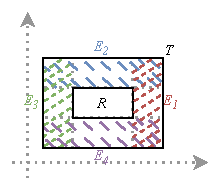
\includegraphics[width=0.4\linewidth]{./img/_rectangle_space.pdf}
            \end{figure}

            Consider the probabilistic event "$x \in E_i$".
            For the training data $x \sim \mathcal{D}$ this holds iff none of those points
            end up in $E_i$ as, if a training point is in $E_i$, $R$ would be bigger to include it and $E_i$ would be smaller.

            Now consider four other regions $F_1, \dots, F_4$ of the plane related to $E_i$ but defined differently
            in such a way that $\mathcal{P}_{x \sim D}[x \in F_i] = \frac{\varepsilon}{4}$.
            This can be achieved by expanding the $E_i$ regions to take some area of the rectangle $R$.
            \begin{figure}[H]
                \centering
                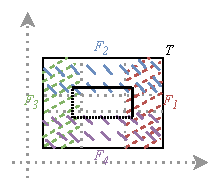
\includegraphics[width=0.4\linewidth]{./img/_rectangle_space2.pdf}
            \end{figure}

            Then, as $E_i$ are smaller than $F_i$, it holds that:
            \[ 
                \begin{split}
                    \mathcal{P}_{x \sim D}[x \in E_i] < \frac{\varepsilon}{4} &\Rightarrow \mathcal{P}_{x \sim D}[x \in (T \smallsetminus R)] < \varepsilon \\
                    & \Rightarrow \text{error}_{\mathcal{D}, T}(R) < \varepsilon
                \end{split}
            \]
            
            \textit{To be continued\dots}
        \end{proof}
    \end{theorem}
\end{example}


\end{document}